\documentclass[a4paper,titlepage]{article}
\usepackage[utf8]{inputenc}
\usepackage{fullpage}
\usepackage{indentfirst}
\usepackage[per-mode=symbol]{siunitx}
\usepackage{listings}
\usepackage{graphicx}
\usepackage{color}
\usepackage{amsmath}
\usepackage{array}
\usepackage[hidelinks]{hyperref}
\usepackage[format=plain,font=it]{caption}
\usepackage{subcaption}
\usepackage{standalone}
\usepackage[nottoc]{tocbibind}
\usepackage[nameinlink]{cleveref}
\usepackage{todonotes}
%equations https://www.rpi.edu/dept/arc/training/latex/LaTeX_symbols.pdf
%TODO: FSM picture
%TODO: keypad pictures

% Custom commands
\newcommand\numberthis{\addtocounter{equation}{1}\tag{\theequation}}
\newcolumntype{P}[1]{>{\centering\arraybackslash}p{#1}}

\title{\textbf{ECSE-426 \\ Microprocessor Systems \\ Report 2}}
\author{
    \textbf{Group 8} \\ \\
    \begin{tabular}{P{4cm} P{4cm}}
    Sean Stappas & Eric Vuong \\
    260639512 & 260630559  \\
    \end{tabular}
}
\date{March XX, 2018}

\begin{document}
\sloppy

\maketitle
\clearpage

\section{Abstract}


\section{Problem Statement}

The objective of lab 3 and 4 was to implement the concepts of timers, PWM, multi-threading, and keypad scanner into a system using the F4 Discovery board. \todo{review after lab 4}. The final deliverable was a voltage generator based on RMS. The system should have the following requirements:

\begin{itemize}
\item The discovery board should provide inputs with a numerical keypad, thus allowing the user to generate a desired voltage no more than \SI{2.8}{\volt} with a good stability.

\item Similar to lab 1 \& 2, the board should be interfaced with a 7-segment display, showing 4 different outputs: RMS Voltage, Min, Max, and user voltage input in the form of X.Y.

\item The system should have 3 modes, controlled by the numerical keypad: sleep mode, input mode (restart) , and display mode. To get into sleep mode, the user will hold the '*' button for more than 3 seconds. During this time, the display should be off with an output voltage 0. Moreover, power consumption of the board should be taken into consideration, such as turning off any unused components. For the restart mode,  the user will have to hold '*' for around 1-2 seconds. Finally, the '\#' button was used to simulate an \textit{Enter} button and '*' was used for the \textit{Delete} button, deleting the last digit entered. Pressing the \textit{Enter} button would get into display phase.

\item Timers should be used generate the PWM and ADC readings. Unlike lab 1-2, a timer would be used to trigger the ADC sampling time.

\item The voltage generator would be controlled using PWM pulse generation, a simple rectifier circuit and a simple control system to adjust the output voltage based on load variations. The reaction time should not take longer than 0.5 seconds. Finally, depending on the pulse frequency chosen, a FIR filter and an analysis on the parameters of the filter would have to be performed to obtain a decent filtering.
\todo{graphs, visual analysis}

\item In lab 4, multi-threading would have to be designed with CMSIS-RTOS while ensuring the same functionalities from lab 3.

\end{itemize}

\section{Theory and Hypothesis}

\subsection{Circuit}
In order to output the desired voltage of a signal, a simple rectifier that would hold the charge in the capacitor, and discharge it with resistive loads. In order to charge and discharge the capacitor, a PWM pulse generator would have to be applied. Finally, the RMS voltage of the charge and discharge cycles should lead to a fairly stable output based on the parameters of the FIR filter.

\begin{figure}[!htb]
  \centering
  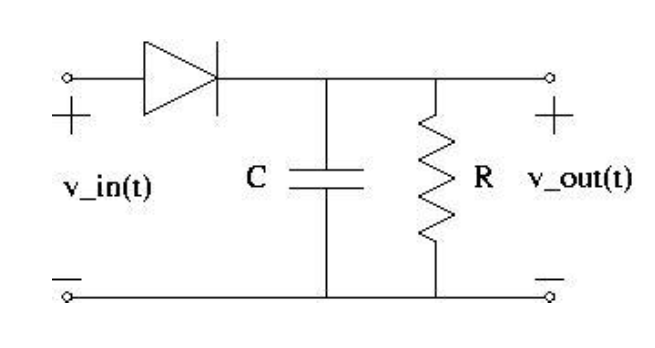
\includegraphics[width=\columnwidth]{figures/rectifier_circuit.png}
  \caption{Simple rectifier circuit with capacitor and resistive load \cite{lab3_handout}.}
  \label{fig:rec_circuit}
\end{figure}

The charge and discharge of a capacitor from \Cref{fig:rec_circuit} was determined by the time constant:

\begin{equation}
\tau = R \times C
\label{eq:time_constant}
\end{equation}

and the charge \eqref{eq:charge} and discharge \eqref{eq:discharge} equation are the following:

\begin{equation}
V_c = V_s (1-e^\frac{-t}{\tau})
\label{eq:charge}
\end{equation}
\begin{equation}
 V_c = V_s \times e^\frac{-t}{\tau}
 \label{eq:discharge}
\end{equation}

Thus, the generated output voltage is dependent on the width of each pulse and the values of the capacitor and resistor, the pulse frequency would have to vary accordingly.

A time triggered ADC would have to be used to obtain the output readings. This part was crucial, because the data would then have to be filtered and fed back into the control system to readjust the duty cycle of the PWM input depending on the load variations. The ADC will also be used with DMA, similar to lab 1-2.
\subsection{Filtering}
The generated DC voltage is often noisy, a FIR filter would be recommended for this lab. Thus, depending on the desired cut-off frequency, filter delay and gain, the order and coefficients of the FIR filter, as explained in lab 1-2, would have to be calculated.
\subsection{Keypad}
For the 4x3 keypad, each pins corresponds to a column or row, for a total of 7 pins, excluding the ground. The buttons on the keypad are wired in a way, such that each button pressed corresponds to the connection between a row and a column on contact. Thus, a scanning algorithm could be implemented to determine the key presses by the user. The configurations of the GPIO pins would be necessary and debouncing measures similar to lab 1-2 would have to be considered.

\subsection{Multi-threading}
As part of lab 4, the aforementioned functionalities would have to be integrated and operating concurrently through the CMSIS-RTOS \todo{RTX-based?} by multi-threading components. In other words, the PWM pulse generator, ADC sampling and controls, and the keypad would be functioning in parallel.

\section{Implementation}
The peripheral configurations of the board were done using the STM32CubeMx software. This helped us speed up the set-up process for time controlled PWM, keypad GPIO pins, 7-segment display pins, and the time triggered ADC with DMA. \Cref{fig:circuit_lab3} shows an overview of the various implementations of the circuit. There were various design constraint that had to be taken into consideration during the implementation.  Similar to lab 1-2, a blue button (push button in \Cref{fig:circuit_lab3}) was used to switch the display settings between the processed RMS voltage, max and min values.

\begin{figure}[!htb]
  \centering
  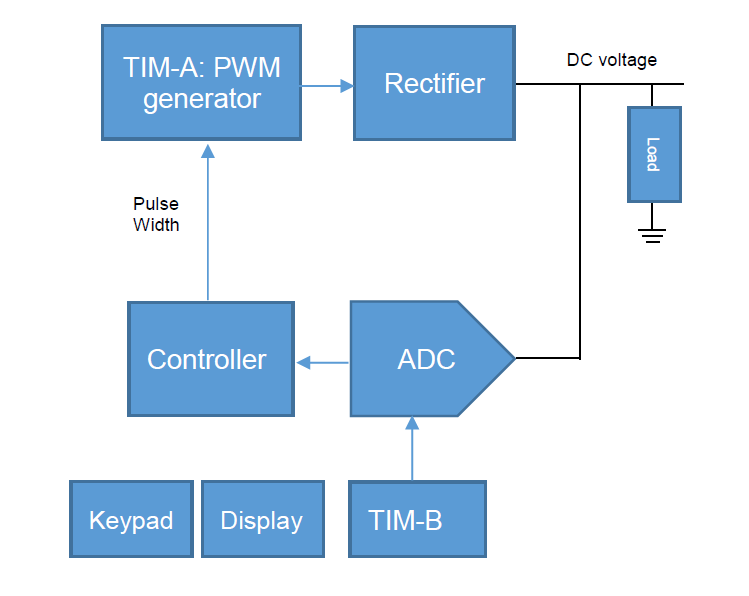
\includegraphics[width=\columnwidth]{figures/high_level_circuit_lab3.png}
  \caption{High level circuit description. \cite{lab3_handout}.}
  \label{fig:circuit_lab3}
\end{figure}

The pinout configuration used can be seen in \todo{update the pin-out}, the details of which would be given in the next sections.

\begin{figure}[!htb]
  \centering
  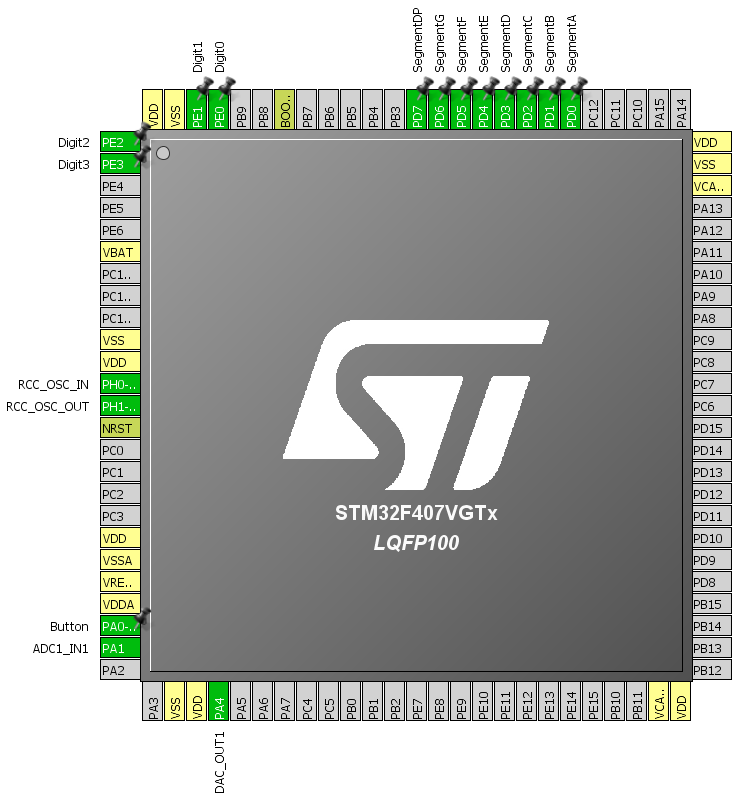
\includegraphics[width=\columnwidth]{figures/pinout.png}
  \caption
  {STM32F4 pinout diagram.}
  \label{fig:pinout}
\end{figure}

\subsection{Keypad}
As aforementioned, the keypad provided for the lab was a 4x3 keypad, with digits ranging from 0-9 with 2 special characters: '*' and '\#'. Since the keypad pins are wired in a way such that each key pressed would connect a row and a column together.

In this way, a scanning algorithm could be used to determine with key was pressed. To do so, we would have to write on the rows and read from the column pins. Moreover, we would be writing to the rows in a specific way and reading from the columns, which are initially set to '0' with the pull-down resistors being used to fix the initial states to be logic '0'. At any instant, only one pin of the 4 columns was set to '1' and the rest were set to '0'. When a button was pressed, only one of the column would turn '1', thus allowing us to determine which row and column has been pressed. This method is effective when the columns and rows were scanned at a fast enough frequency, such that duration of a button pressed lasts an entire scan cycle. Similar to lab 1-2, a debouncer has been implemented whenever a new button is pressed.

\subsection{Timer Triggered ADC with DMA}
A TIM peripheral timer could be used to trigger ADC readings. Some configurations were needed to setup the ADC to be triggered with timers. The ADC would need an external source, such as a timer to trigger the ADC for a new conversion. However, doing so would require the user to wait for the end of conversion before reading the data. Note that timers also has channels to use in PWM mode, generating pulse on a GPIO pin, which will be discussed later. When reading from the ADC, it was important to set the correct timer frequency. The timer would have to be triggering the ADC at a rate faster than the PWM pulses.  \todo {did we have any issue, with the timer being too fast?}. The frequency of the timer was calculated with the specific bus clock value of the timer, prescaler and period value as follows:

%TODO: timer and ext trigger configuration on STMCube.
\begin{equation}
Desired Timer Frequency = \frac{Bus Clock Frequency}{Prescale \times Period }
\end{equation}


The ADC sampling rate was set at \todo{checklab}

\subsection{PWM Pulse Generation with Timer and Rectifier Circuit}
\Cref{fig:rec_circuit} shows the circuit implemented in the lab. The capacitor value chosen was \SI{1}{\micro\farad} and the resistor value was \SI{4.7}{\kilo\ohm}. This yields a time constant of \SI{4.7}{\milli \second}.

In order to properly generate the desired voltage, the pulse period would have to be smaller than the time constant. During the charging phase, the RC circuit driven by the step function of the PWM, thus charging to a certain voltage level. During the discharge phase, since there is no external voltage being applied, the system's voltage response is due solely by the discharge of the capacitor \cite{pwm_rc_citation}. If the period of the pulse is relatively large, the range of voltage generated would be less, as the gap between each duty cycle is too big and the discharge will happen too quickly, thus leading to a \SI{0}{\volt} output. Likewise, if the duty cycle is too large, the charging phase last long enough, such that the output voltage will be the \SI{3}{\volt}. The pulse period was chosen to be \SI{10}{\kilo \hertz}.


\todo{is this true}The pulse width had 8400 steps, thus allowing a lot of resolution to the output voltage. A control has been applied so that any variations in the resistor value could be readjusted by changing the pulse width. To do so, at every sampling rate, the pulse width adjustment would be calculated based on the difference of the desired voltage and output ADC reading as follows:
\begin{equation}
Voltage Difference = Desired Voltage - Current ADC Voltage Reading
\label{eq:voltage_difference}
\end{equation}
Depending on the voltage difference from \eqref{eq:voltage_difference}, an incremental or decremental pulse width would be applied to the current pulse width. this incremental or decremental pulse width would is proportional to the voltage difference. In order to speed up the reaction time, the pulse width applied can be increased if the voltage difference is relatively high. Thus, a function to compensate the charging and discharging delay of the RC circuit would have helped speed up the reaction time. In other words, a P-controller was applied and alternate controllers could have applied to improve the reaction time, such as PID controller.

\begin{figure}[!htb]
  \centering
  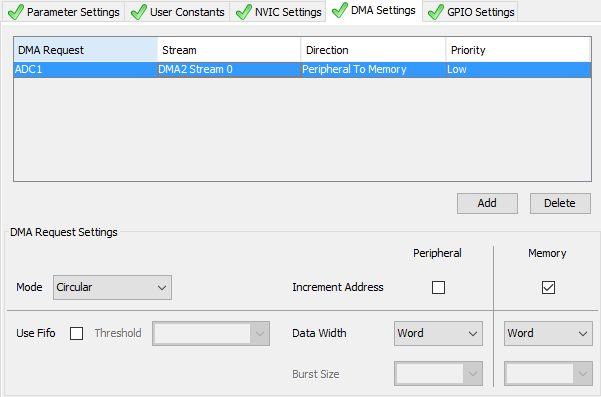
\includegraphics[width=\columnwidth]{figures/adc_config_dma.png}
  \caption{ADC DMA configuration.}
  \label{fig:adc_config_dma}
\end{figure}

The ADC was also configured to use continuous DMA requests as seen in \Cref{fig:adc_config_dma}. This allows for much simpler reading of the voltage values from a location in memory, with the trade-off of having unnecessary conversion take place.


\subsection{Filtering \& Processing}

Since it is required to filter out the high frequency from the PWM generator to obtain a stable DC voltage, a linear-phase filter with symmetrical coefficients FIR filter, similar to prior lab with order 10 has been used. The raw data to be filtered was stored in a vector of size 10. Every new sampling datum, the oldest was discarded, and thus the FIR would filter the newly formed vector to output the filtered data to the display.

\subsection{System State Transistions}
With the keypad implemented, the functionality of the board had to be functioning in 3 different modes: sleep mode, input mode, and display mode. Thus, a state transistion had to be implemented. The following \Cref{fig:state_transitions} shows the various state transistions triggered by key presses from the user.

\begin{figure}[!htb]
  \centering
  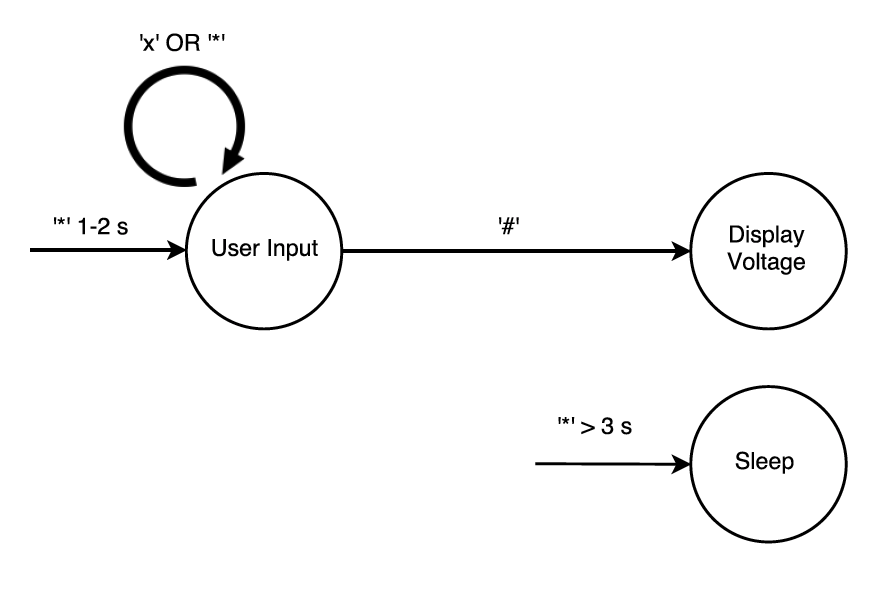
\includegraphics[width=\columnwidth]{figures/state_transitions.png}
  \caption
  {The state transistions of the system.}
  \label{fig:state_transitions}
\end{figure}

\subsection{Sleep mode \& Power Consumptions}
% TODO: cite the Book

One of the benefits of using a Cortex -M microcontrollers is that they are power efficient \cite{yiu}. Moreover, the STM32CubeMx provided us with power consumption measurement tools. Thus, it was easier to make the board as power efficient as possible in the sleep phase. Thus, the ADC, PWM, 7-segment GPIOS and timers were turned off. In the multi-threaded implementation, which will be discussed later, all the above mentioned threads were terminated.
\todo{Sean, could you maybe elaborate a bit on this one, if there were some tricks on the STM32CubeMx regarding power consumption}


\subsection{7-Segment Display}
The same 7-segment display configurations from lab 1 and 2 were used for this lab. However, in the user input phase, the display is modified, such that the second and third digits from the left will display the user input voltage. Upon pressing enter, the display would go back to the normal display mode (YX.XX), where Y is the display mode and X is the desired value in floating points. \Cref{fig:7_segment} shows the meaning of each pin, which has been tested by applying a high voltage and grounding each pin through trial and error in the lab.
\begin{figure}[!htb]
  \centering
  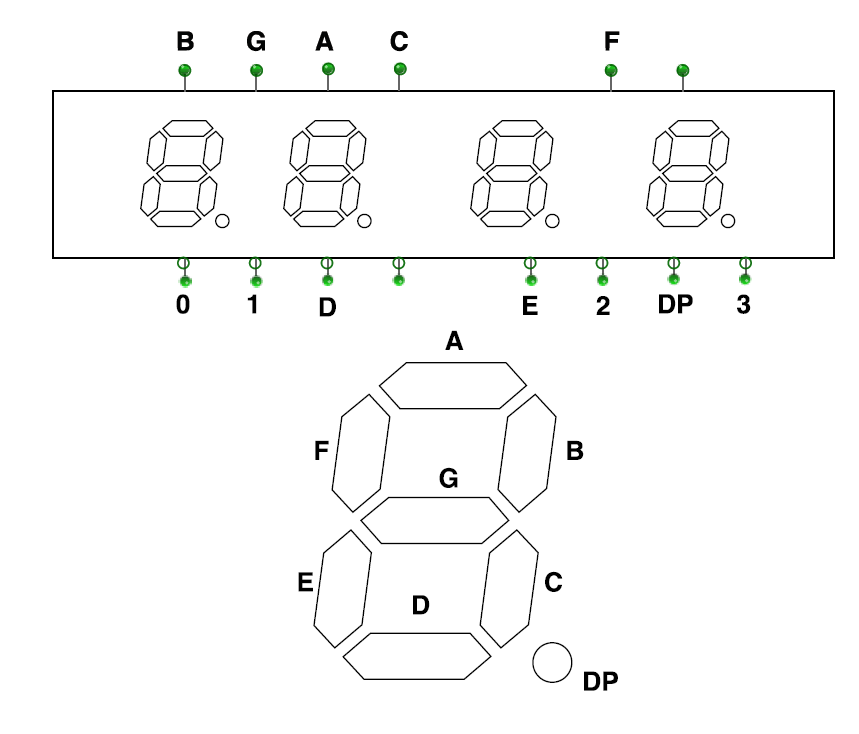
\includegraphics[width=\columnwidth]{figures/7seg_display.PNG}
  \caption
  {Meaning of pins on 7 segment display. Numbers 0 to 3 represent the 4 digits from left to right. The letters represent segments, as shown in the bottom of the figure. DP represents the decimal point.}
  \label{fig:7_segment}
\end{figure}

For reference, the display mode of operations (RMS, Max, Min) were represented by the first digit of the 7-segment display was used. The RMS, Max and Min modes are thus represented by digits 0, 1 and 2, respectively. In each mode, the remaining 3 digits represent the desired number, with two decimal places.

\section{Testing and Observations}

\section{Conclusion}
In conclusion, a voltmeter was built using the STM32F407VGTx. The display board was able to properly display the desired values without any flickers or obvious transitions. The voltmeter was able to successfully read the data and an error of less than 5\% is observed. Also, the user was able to switch between different modes (RMS, max and min), where the max and min would update only once every 10 seconds.

Many improvements could be made to our design and method. For example, to represent our input vector, we used a simple array structure with shifting of values at each new datum. However, since it is essentially a FIFO queue, a linked list structure would be more appropriate and efficient. An improvement to our testing method would be to generate more interesting voltage signals. Indeed, we simply generated DC voltages, but it would have been interesting to generate more complex AC signals, such as a sine wave, and validate that the correct RMS, max and min values are captured.


% \begin{figure}[!htb]
%   \centering
%   \includegraphics[width=\columnwidth]{schematics/diff_amp_passive.pdf}
%   \caption[Differential amplifier with passive load schematic.]
%   {Schematic for the differential amplifier with passive load.}
%   \label{fig:diff_passive_schematic}
% \end{figure}

% \begin{table}[!htb]
% \small
% \centering
% \caption[Differential amplifier with active load DC currents.]
% {Inferred DC currents compared to simulated DC currents in the differential with active load.}
% \label{tab:dc_curr_active}
% \begin{tabular}{|c|c|c|} \hline
% \textbf{Resistor}&\textbf{Inferred (mA)}&\textbf{Simulated (mA)}\\ \hline
% $R_1$&0.265&0.266\\\hline
% $R_2$&0.309&0.263\\\hline
% $R_3$&0.300&0.264\\\hline
% $R_4$&0.127&0.131\\\hline
% $R_5$&0.127&0.131\\\hline
% \end{tabular}
% \end{table}


\clearpage
\onecolumn
\appendix

\bibliography{bibliography.bib}{}
\bibliographystyle{IEEEtran}


\end{document}
